%%%%%%%%%%%%%%%% NÃO ALTERE O CAMPO ABAIXO 
\documentclass[10pt,twoside,a4paper]{article}
\usepackage[T1]{fontenc}
\usepackage[utf8]{inputenc}
\usepackage[portuges]{babel}
\usepackage[a4paper]{geometry}
\geometry{tmargin=1.2cm,bmargin=1.7cm,lmargin=1.5cm,rmargin=1.5cm}
\usepackage{graphicx}
\usepackage{indentfirst}
\usepackage{subcaption} % figuras lado a lado
\usepackage{booktabs} %tabelas
\usepackage{url}% web links
\usepackage{semat}
\usepackage{lipsum} %Texto automático
\usepackage{amsthm, amsmath, amssymb, wasysym, MnSymbol}
%%%%%%%%%%%%%%%%

%%%%%%%%%%%%%%%% Se necessitar de pacotes adicionais insira abaixo
%\usepackage[•]{•}
%%%%%%%%%%%%%%%%%%%%%%%%%%%%%%%%

%%%%%%%%%%%%%%%%%%
% Evite redefinir ou criar comandos, por exemplo:
% \R=\mathbb{R} ,\newtheorem{teo}{Teorema}, etc
% Isto pode gerar conflito quando os trabalhos forem
% compilados juntos para o caderno de resumos
\newtheorem{theorem}{Teorema}
\newtheorem{proposition}[theorem]{Proposição}
\newtheorem{lemma}[theorem]{Lema}
\newtheorem{definition}[theorem]{Definição}
\newtheorem{corollary}[theorem]{Corolário}
\renewcommand{\qedsymbol}{$\blacksquare$}
\renewcommand{\sin}{{\rm{sen}\hspace{2pt}}}
\renewcommand{\sinh}{{\rm{senh}\hspace{2pt}}}
%%%%%%%%%%%%%%

%%%%%%%%%%% Não altere os comandos abaixo
\newcommand*{\affaddr}[1]{#1} 
\newcommand*{\affmark}[1][*]{\textsuperscript{#1}}
\newcommand*{\email}[1]{\texttt{#1}}
\usepackage{helvet}% Fonte 
\renewcommand{\familydefault}{\sfdefault}% Fonte 
\renewcommand\Authands{ e }
\evento{XVIII Semat e VIII Semest}
\date{02 a 05 de outubro de 2018}
%%%%%%%%%%%%%%%%






% Dados do trabalho
\title{Análise numérica da equação da difusão bidimensional em regime transiente pelo método explícito}
% Autores: o primeiro será, necessariamente, o apresentador do trabalho
\author[1]{\underline{Felipe José Oliveira Ribeiro }\thanks{feliperibeiro.ufu@gmail.com}}
\author[1]{Ítalo Augusto Magalhães de Ávila\thanks{italo.ufuracing@gmail.com}}
\author[1]{Hélio Ribeiro Neto\thanks{helio.ribeiro@ufu.br}}
\author[1]{Aristeu da Silveira Neto\thanks{aristeus@ufu.br}}
\affil[1]{FEMEC - Universidade Federal de Uberlândia}


%palavras-chave: insira até três palavras
\keywords{Análise numérica. Difusão bidimensional transiente. Diferenças finitas.}

%Compilar o arquivo com PDFLatex
%---------------------------------------------------
\begin{document}
	\inserirtitulo
	\linespread{1.5}% Espaçamento 1.5
	%==================================
	% RESUMO
	%==================================
	
	\section{Resumo}
	No presente trabalho realizar-se-á um estudo de caso do erro numérico na solução da EDP que modela o processo de difusão bidimensional de uma dada informação. 
	
	
	%==================================
	% INTRODUÇÃO
	%==================================
	\section{Introdução} % apague as linhas abaixo e insira aqui a introdução
	
	Muitos fenômenos físicos podem ser modelados, isto é, representados matematicamente, por meio de Equações Diferenciais Parciais (EDPs). A sua solução por métodos analíticos, no entanto, é limitada a casos lineares e simples, que não representam de maneira satisfatória a maioria dos fenômenos físicos. O método numérico é empregado como alternativa para a solução de problemas de maior complexidade. Um exemplo é a solução da equação da energia térmica em regime transiente. Na literatura da área, existem vários métodos de solução numérica de equações diferenciais. São exemplos o Método dos Elementos Finitos, Método dos Volumes Finitos e Método de Diferenças Finitas. Em tais métodos, o domínio é discretizado e as relações diferenciais são aproximadas por um sistema  algébrico de equações. Tal aproximação implica em um erro em relação à solução exata, o qual pode ser quantificado sob determinadas condições. No presente trabalho, procura-se apresentar um estudo de caso para a análise de erro envolvendo a resolução da EDP que modela a equação da energia térmica em um domínio bidimensional. 
	
	%Muitos fenômenos físicos são modelados, isto é,  representados matematicamente, por meio de Equações Diferenciais Parciais (EDP), as quais em sua grande maioria só tem solução via métodos de resolução numérica. Um exemplo é a solução da equação da energia térmica em regime transiente. As técnicas de resolução analíticas são limitadas para resolver tais equações. São exemplos de fatores de limitação, a geometria do domínio, os tipos de condição de fronteira e a presença de termos não lineares na equação. Na literatura da área, existem vários métodos de solução numérica de equações diferenciais. São exemplos o Método dos Elementos Finitos, Método dos Volumes Finitos e Método de Diferenças Finitas. Tais métodos, em essência, no processo de solução transformam as equações apresentadas na forma contínua em uma forma algébrica. Esse processo recebe o nome de discretização. A equação gerada pela discretização é uma aproximação da equação original e, portanto, apresenta erro, o qual pode ser quantificado sob determinadas condições. No presente trabalho, procura-se apresentar um estudo de caso para a análise de erro envolvendo a resolução da EDP que modela a equação da energia térmica. 
	
	%==================================
	% Primeira Seção
	%==================================
	\section{Método numérico} % apague as linhas abaixo e insira aqui a primeira seção
	
	Na equação da difusão, para o caso bidimensional (indicada abaixo), aparecem duas parcelas diferenciais \cite{Leveque_parabolic}. 
	\begin{equation} \label{difusao_pura}
	\frac{\partial \phi}{\partial t} = \alpha \,\left( \frac{\partial^{2} \phi}{\partial x^{2}} + \frac{\partial^{2} \phi}{\partial y^{2}} \right) 
	\end{equation}
	Na qual $\phi$ é a variável a ser transportada, função do tempo $t$ e das variáveis espaciais $x$ e $y$, $\alpha$ é uma constante, a qual pode representar o coeficiente de difusividade de uma dada informação.
	Utilizando a expansão em série de Taylor (equação \ref{serie_taylor}), é possível discretizar os termos no tempo e no espaço para a resolução numérica do problema. 
	
	\begin{equation} \label{serie_taylor}
	\phi \left(t+\Delta t, x, y \right)= \phi \left(t, x, y\right) + \sum\limits_{n=1}^{\infty} \frac{\Delta t^{n}}{n!} \frac{\partial^{n} \phi \left(t, x, y\right)}{\partial t^{n}}.
	\end{equation}
	Para a discretização do termo diferencial de primeira ordem, faz-se uso da equação acima para a expansão da função no domínio do tempo:
	
	\begin{equation} \label{Time_discretization}
	\frac{\phi \left(t+\Delta t, x, y \right)-\phi \left(t, x, y\right)}{\Delta t}= \frac{\partial \phi \left(t, x, y\right)}{\partial t} + \sum\limits_{n=2}^{\infty} \frac{\Delta t^{n-1}}{n!} \frac{\partial^{n} \phi\left(t, x, y\right)}{\partial t^{n}}.
	\end{equation}
	Truncando a equação \ref{Time_discretization} no termo de primeira ordem ($\mathcal{O}(\Delta t)$), obtém-se o método de Euler explícito.
	Analogamente, a discretização para os termos de segunda ordem é obtida, fazendo uso de um incremento e um decremento no espaço, enquanto o tempo é fixado.
	
	\begin{equation} \label{Spacial_discretization1}
	\phi \left(t, x+\Delta x, y\right)= \phi \left(t, x, y\right) \\
	+\sum\limits_{n=1}^{\infty} \frac{\Delta x^{\left(2n-1\right)}}{\left(2n-1\right)!} \frac{\partial^{\left(2n-1\right)} \phi \left(t, x, y\right)}{\partial x^{\left(2n-1\right)}}\\
	+\sum\limits_{n=1}^{\infty} \frac{\Delta x^{\left(2n\right)}}{\left(2n\right)!} \frac{\partial^{\left(2n\right)} \phi \left(t, x, y\right)}{\partial x^{\left(2n\right)}},
	\end{equation}
	
	\begin{equation} \label{Spacial_discretization2}
	\phi \left(t, x-\Delta x, y \right)= \phi \left(t, x, y\right) \\
	-\sum\limits_{n=1}^{\infty} \frac{\Delta x^{\left(2n-1\right)}}{\left(2n-1\right)!} \frac{\partial^{\left(2n-1\right)} \phi \left(t, x, y\right)}{\partial x^{\left(2n-1\right)}}\\
	+\sum\limits_{n=1}^{\infty} \frac{\Delta x^{\left(2n\right)}}{\left(2n\right)!} \frac{\partial^{\left(2n\right)} \phi \left(t, x, y\right)}{\partial x^{\left(2n\right)}}.
	\end{equation}
	Somando as equações \ref{Spacial_discretization1} e \ref{Spacial_discretization2}, obtém-se a discretização para a derivada segunda em uma das direções. 
	
	\begin{equation} \label{Spacial_discretization3}
	\frac{\phi \left(t, x+\Delta x, y\right)-2 \phi \left(t, x, y\right) + \phi \left(t, x-\Delta x\right)}{\Delta x^2} = \\
	\frac{\partial^{2} \phi \left(t, x, y\right)}{\partial x^{2}}+ \\
	2 \sum\limits_{n=2}^{\infty} \frac{ \Delta x^{\left(2\left(n-1\right)\right)}}{\left(2n\right)!} \frac{\partial^{\left(2n\right)} \phi \left(t, x, y\right)}{\partial x^{\left(2n\right)}}.
	\end{equation}
	A mesma metodologia empregada em $x$ é estendida à dimensão $y$.
	Substituindo as relações truncadas na equação \ref{difusao_pura} tem-se a equação \ref{difusao_discretizada} .
	\begin{equation} \label{difusao_discretizada}
	\begin{split}
	\frac{\phi \left(t+\Delta t, x, y\right)-\phi \left(t, x, y\right)}{\Delta t} \ - \ &\alpha \left( \frac{\phi \left(t, x+ \Delta x, y \right)-2 \phi \left(t, x, y \right) + \phi \left(t, x- \Delta x, y \right)}{\Delta x^2} \right) -\\
	&\alpha \left( \frac{\phi \left(t, x, y+ \Delta y \right)-2 \phi \left(t, x, y \right) + \phi \left(t, x, y- \Delta y \right)}{\Delta y^2} \right) \approx 0 .% + g\left(x,t\right)
	\end{split}
	\end{equation}
	
	% comentar aqui
	
	A solução numérica requer a discretização dos domínios espacial e temporal. Ou seja, deve-se traduzir um
	conjunto contínuo e infinito de informações em um conjunto discreto e finito, no qual é empregada a metodologia numérica. Os domínios espacial e temporal são discretizados uniformemente. Assim, para $(t,x,y) \in [a,b] \times [c,d] \times [e,f]$, tem-se:
	
	\vspace*{-3mm}
	
	\begin{equation} \label{discretizacao_tempo_espaco}
	t^{N} = N \Delta t, \ \ N=0,1,2,...,M,
	\end{equation}	
	
	\begin{equation}
	x_{I} = I \Delta x, \ \ I=0,1,2,...,L,
	\end{equation}
	
	\begin{equation}
	y_{J} = J \Delta y, \ \ J=0,1,2,...,O,
	\end{equation}
	onde $M$, $L$ e $O$ são o número de divisões nos intervalos $[a,b]$, $[c,d]$ e $[e,f]$, respectivamente.	
	
	É conveniente definir a solução numérica para os pontos discretos $\Phi_{I,J}^{N}$, que não é idêntica à solução analítica de $\phi (x,y,t)$. Assim, é possível reescrever a equação \ref{difusao_discretizada} como indicado à
	seguir.
	
	
	\begin{equation} \label{numerical_sol}
	\begin{split}
	\frac{\Phi_{I,J}^{N+1}-\Phi_{I,J}^{N} }{\Delta t} - \alpha \left( \frac{\Phi_{I+1,J}^{N} -2 \Phi_{I,J}^{N} + \Phi_{I-1,J}^{N}}{\Delta x^2} \right) -	\alpha \left( \frac{\Phi_{I,J+1}^{N}-2 \Phi_{I,J}^{N} + \Phi_{I,J-1}^{N}}{\Delta y^2} \right) = 0. % + g\left(x,t\right)
	\end{split}
	\end{equation}
	
	Para a análise do erro, parte-se para a formulação de uma equação modificada, que descreve qual equação contínua a equação \ref{numerical_sol} modela sem erros. Define-se uma função $\psi(t,x,y)$ que é contínua e coincidente com a solução no ponto discreto ($N,I,J$) e é diferente da solução exata $\phi(t,x,y)$. Em outras palavras, $\phi(t,x,y)$ é a solução exata, $\Phi_{I,J}^{N}$ é a solução aproximada, obtida do sistema discreto, e $\psi(t,x,y)$ é a solução contínua que está de acordo com a obtida por $\Phi$ no ponto (respectivos $N$, $I$ e $J$) e que é diferente de $\phi(t,x,y)$. Substituindo $\Phi_{I,J}^{N}$ na equação \ref{numerical_sol} por $\psi(t,x,y)$ e expandindo os termos em série de Taylor ao redor do ponto $(t,x,y)$, obtém-se a equação apresentada à seguir.	
	
	\begin{equation} \label{difusao_continuum}
	\begin{split}
	&\frac{\partial \psi}{\partial t} - \alpha \left( \frac{\partial^{2} \psi}{\partial x^{2}} + \frac{\partial^{2} \psi}{\partial y^{2}} \right) = 2 \alpha \sum\limits_{n=2}^{\infty} \frac{ \Delta x^{\left(2\left(n-1\right)\right)}}{\left(2n\right)!} \frac{\partial^{\left(2n\right)} \psi \left(t, x, y\right)}{\partial x^{\left(2n\right)}} + 2 \alpha \sum\limits_{n=2}^{\infty} \frac{ \Delta y^{\left(2\left(n-1\right)\right)}}{\left(2n\right)!} \frac{\partial^{\left(2n\right)} \psi \left(t, x, y\right)}{\partial y^{\left(2n\right)}} - \sum\limits_{n=2}^{\infty} \frac{\Delta t^{n-1}}{n!} \frac{\partial^{n} \psi\left(t, x, y\right)}{\partial t^{n}}. % + g\left(x,t\right)
	\end{split}
	\end{equation}
	O lado direito da equação \ref{difusao_continuum} expressa o erro numérico da discretização segundo a metodologia explícita. Tal relação é apresentada em função de termos espaciais e temporais. Visando facilitar a análise, procura-se reescrever a relação em função apenas de termos do domínio espacial. A equação \ref{difusao_pura} não pode ser empregada, no entanto, para suprimir termos de ordens elevadas [2], já que a relação dada em (\ref{difusao_continuum}) descreve a solução discretizada, que se difere da exata. Assim, deve-se empregar sistematicamente a equação \ref{difusao_continuum} na simplificação dos termos desejados. 
	
	Truncando termos de ordem superior a 4 tem-se:
		
	\begin{equation} \label{difusao_continuum2}
	\frac{\partial \psi}{\partial t} - \alpha \left(\frac{\partial^{2} \psi}{\partial x^{2}} + \frac{\partial^{2} \psi}{\partial y^{2}} \right) + \frac{\Delta t}{2} \frac{\partial^{2} \psi}{\partial t^{2}} + \frac{\Delta t^{2}}{6} \frac{\partial^{3} \psi}{\partial t^{3}} - \alpha \frac{\Delta x^{2}}{12} \frac{\partial^{4} \psi}{\partial x^{4}} - \alpha \frac{\Delta x^{4}}{60} \frac{\partial^{6} \psi}{\partial x^{6}} - \alpha \frac{\Delta y^{2}}{12} \frac{\partial^{4} \psi}{\partial y^{4}} - \alpha \frac{\Delta y^{4}}{60} \frac{\partial^{6} \psi}{\partial y^{6}} +  ... = 0.
	\end{equation}
	Derivando parcialmente a equação \ref{difusao_continuum2} no domínio do tempo, multiplicando a equação resultante por $(-\Delta t/2)$ e somando-a à primeira, tem-se a equação indicada abaixo.
	
	\begin{equation} \label{termo_temporal_dois}
	\begin{split}
	\frac{\partial \psi}{\partial t} - \alpha \left(\frac{\partial^{2} \psi}{\partial x^{2}} + \frac{\partial^{2} \psi}{\partial y^{2}} \right) - \frac{\Delta t^{2}}{12} \frac{\partial^{3}\psi}{\partial t^{3}} + \alpha \Delta t \frac{\partial^{3} \psi}{\partial x^{2} \partial t} + \alpha \Delta t \frac{\partial ^{3} \psi}{\partial y^{2} \partial t} + \alpha \frac{\Delta x^{2} \Delta t}{2} \frac{\partial^{5} \psi}{\partial x^{4} \partial t} + \alpha \frac{\Delta y^{2} \Delta t}{2} \frac{\partial^{5} \psi}{\partial y^{4} \partial t} ... = 0.
	\end{split}
	\end{equation}	
	O mesmo procedimento é aplicado até a segunda ordem para a dimensão $t$, multiplicando o resultado por $(\Delta t^{2}/12)$ e somando-o à equação \ref{termo_temporal_dois}, de forma a suprimir o termo $ \frac{\Delta t^{2}}{12} \frac{\partial^{3}\psi}{\partial t^{3}}$. A resultante é indicada à seguir.
	
	\begin{equation} \label{termo_temporal_tres}
	\begin{split}
	&\frac{\partial \psi}{\partial t} - \alpha \left(\frac{\partial^{2} \psi}{\partial x^{2}} + \frac{\partial^{2} \psi}{\partial y^{2}} \right) +\frac{\Delta t^{3}}{12} \frac{\partial^{4}\psi}{\partial t^{4}} + \frac{\Delta t^{4}}{2(6!)} \frac{\partial^{5}\psi}{\partial t^{5}}- 2 \frac{\alpha \Delta x^{2}}{4!} \frac{\partial^{4} \psi}{\partial x^{4}} - 2 \frac{\alpha \Delta y^{2}}{4!} \frac{\partial^{4} \psi}{\partial y^{4}} - 2 \frac{\alpha \Delta x^{4}}{6!} \frac{\partial^{6} \psi}{\partial x^{6}} - \\
	&2 \frac{\alpha \Delta y^{4}}{6!} \frac{\partial^{6} \psi}{\partial y^{6}} - \alpha \frac{\Delta t}{2} \frac{\partial^{3} \psi}{\partial x^{2} \partial t} + \alpha \frac{\Delta t}{2} \frac{\partial^{3} \psi}{\partial y^{2} \partial t} - \frac{\Delta x^{2} \Delta t}{48} \frac{\partial^{4} \psi}{\partial x^{4} \partial t} - \frac{\Delta y^{2} \Delta t}{48} \frac{\partial^{4} \psi}{\partial y^{4} \partial t}  +... = 0.
	\end{split}
	\end{equation}	
	Para cancelar as derivadas parciais nas duas dimensões, faz-se uso do teorema de Clairaut-Schwarz (inversão da ordem de derivação). Essa metodologia deve ser empregada até que todas as derivadas parciais no tempo sejam suprimidas da equação truncada. Por fim, chega-se a equação modificada, que é apresentada abaixo.
	
	\begin{equation} \label{termo_temporal_quatro}
	\begin{split}
	&\frac{\partial \psi}{\partial t} - \alpha \left(\frac{\partial^{2} \psi}{\partial x^{2}} + \frac{\partial^{2} \psi}{\partial y^{2}} \right) = 2\alpha \left(\frac{\Delta x^{2}}{4!} +\frac{\alpha \Delta t}{4}\right) \frac{\partial^{4}\psi}{\partial x^{4}} +2\alpha \left(\frac{\Delta y^{2}}{4!} +\frac{\alpha \Delta t}{4}\right) \frac{\partial^{4}\psi}{\partial y^{4}} + 2\alpha \left(\frac{\Delta x^{4}}{6!} - \frac{\alpha \Delta x^{2}\Delta t}{2(4!)} + \frac{\alpha \Delta x^{4}\Delta t}{48}\right) \frac{\partial^{6}\psi}{\partial x^{6}} + \\
	&2\alpha \left(\frac{\Delta y^{4}}{6!} - \frac{\alpha \Delta y^{2}\Delta t}{2(4!)} + \frac{\alpha \Delta y^{4}\Delta t}{48}\right) \frac{\partial^{6}\psi}{\partial y^{6}} + 2 \alpha \left(\frac{\Delta x^{6}}{8!} - \frac{\alpha \Delta x^{4}\Delta t}{2(6!)} + \frac{\alpha \Delta x^{6}\Delta t}{48(4!)} \right) \frac{\partial^{8}\psi}{\partial x^{8}} + 2 \alpha \left(\frac{\Delta y^{6}}{8!} - \frac{\alpha \Delta y^{4}\Delta t}{2(6!)} + \frac{\alpha \Delta y^{6}\Delta t}{48(4!)} \right) \frac{\partial^{8}\psi}{\partial y^{8}} + ...
	\end{split}
	\end{equation}	
	Ainda, é possível substituir o passo temporal pelo passo espacial. Define-se uma constante $CFL$ [3], que relaciona o passo temporal aos passos espaciais.
	\begin{equation} \label{CFL_one}
	\Delta t = \frac{CFL}{\alpha} min[\Delta x^{2}, \Delta y^{2} ] \ \ \ \ \ 
	\end{equation}
	Substituindo tal condição na equação \ref{termo_temporal_quatro}, tem-se:
	\begin{equation} \label{equacao_modificadaCFL}
	\begin{split}
	\frac{\partial \psi}{\partial t} - \alpha \left(\frac{\partial^{2} \psi}{\partial x^{2}} + \frac{\partial^{2} \psi}{\partial y^{2}} \right) = &2\alpha \left(\frac{\Delta x^{2}}{4!} +\frac{CFL \left[min(\Delta x^{2},\Delta y^{2})\right]}{4}\right) \frac{\partial^{4}\psi}{\partial x^{4}} +2\alpha \left(\frac{\Delta y^{2}}{4!} +\frac{CFL \left[min(\Delta x^{2},\Delta y^{2})\right]}{4}\right) \frac{\partial^{4}\psi}{\partial y^{4}} +\\
	&2\alpha \left(\frac{\Delta x^{4}}{6!} - \frac{CFL \left[min(\Delta x^{2},\Delta y^{2})\right] \Delta x^{2} }{2(4!)} + \frac{CFL \left[min(\Delta x^{2},\Delta y^{2})\right]\Delta x^{4}}{2(4!)}\right) \frac{\partial^{6}\psi}{\partial x^{6}} + \\
	&2\alpha \left(\frac{\Delta y^{4}}{6!} - \frac{CFL \left[min(\Delta x^{2},\Delta y^{2})\right] \Delta y^{2}}{2(4!)} + \frac{CFL \left[min(\Delta x^{2},\Delta y^{2})\right] \Delta y^{4}}{48}\right) \frac{\partial^{6}\psi}{\partial y^{6}} + ...
	\end{split}
	\end{equation}
	Reescrevendo a equação acima de forma conveniente, truncando os termos de ordem superior à quatro, chega-se a equação modificada:


	\begin{equation} \label{equacao_modificadaCFL2}
	\begin{split}
	&\frac{\partial \psi}{\partial t} - \alpha \left(\frac{\partial^{2} \psi}{\partial x^{2}} + \frac{\partial^{2} \psi}{\partial y^{2}} \right) = \frac{\alpha \Delta x^{2}}{12} \frac{\partial^{4} \psi}{\partial x^{4}} + \frac{\alpha \Delta y^{2}}{12} \frac{\partial^{4} \psi}{\partial y^{4}} + \alpha \ CFL \left[min(\Delta x^{2}, \Delta y^{2})\right] \left(\frac{1}{2} \frac{\partial^{4} \psi}{\partial x^{4}} + \frac{1}{2} \frac{\partial^{4} \psi}{\partial y^{4}} + \frac{1}{4}\frac{\partial^{4} \psi}{\partial x^{2} \partial y^{2}} + \frac{1}{4} \frac{\partial^{4} \psi}{\partial y^{2} \partial x^{2}} \right) + \\ &\frac{2 \alpha \Delta x^{4}}{6!} \frac{\partial^{6} \psi}{\partial x^{6}} + \frac{2 \alpha \Delta y^{4}}{6!} \frac{\partial^{6} \psi}{\partial y^{6}} + \alpha CFL \left[min(\Delta x^{2}, \Delta y^{2})\right]  \left(\frac{\Delta x^{2}}{4!} \frac{\partial^{6} \psi}{\partial x^{6}} + \frac{\Delta y^{2}}{4!} \frac{\partial^{6} \psi}{\partial y^{6}} + \frac{\Delta x^{2}}{2(4!)} \frac{\partial^{6} \psi}{\partial x^{4} \partial y^{2}} + \frac{\Delta y^{2}}{2(4!)} \frac{\partial^{6} \psi}{\partial x^{4} \partial y^{2}}\right).
	\end{split}
	\end{equation}
	
	Analisando a equação \ref{equacao_modificadaCFL2}, que apresenta os termos de menores (e mais significativas) ordens do erro numérico, pode-se inferir que o erro é proporcional à condição de $CFL$. Ou seja, o erro é ampliado em função do aumento de tal parâmetro.
	
	%\pagebreak
	
	%==================================
	% Segunda Seção
	%==================================
	\section{Estudo de caso} % apague as linhas abaixo e insira aqui a segunda seção
	
	Para a solução da equação \ref{numerical_sol} é necessário definir o domínio, condições inicial e de contorno e tempo final de simulação. O domínio espacial escolhido foi de $x=[0,2\pi]$ e $y=[0,2\pi]$ e o tempo final de simulação foi de $10$ segundos.
	Para esse estudo de caso, a condição inicial imposta foi:
	\begin{equation} \label{condicao_inicial}
	\Phi(0,x,y)=U_0 \sin\left(\theta x\right) \sin\left(\theta y\right), %e^{-\alpha \theta^2 t},
	\end{equation}
	na qual $U_0$ é a amplitude da função e $\theta$ é o número de onda. As condições de contorno foram:
	\begin{equation} \label{condicoes_contorno}
	\Phi(t,0,y)=0, \ \ \ \Phi(t,2\pi,y)=0,  \ \ \ \Phi(t,x,0)=0, \ \ \ \Phi(t,x,2\pi)=0.
	\end{equation}
	Para determinar o erro e a convergência do método, comparou-se a solução numérica com a solução analítica:
	\begin{equation} \label{solucao_analitica}
	\phi(t,x)=U_0 \sin\left(\theta x\right) \sin\left(\theta y\right) e^{-2 \alpha \theta^2 t}.
	\end{equation}
	Os valores das variáveis $U_0$, $\theta$ e $\alpha$ devem ser escolhidos em função do problema que se deseja resolver. No presente trabalho, o valor escolhido para as três variáveis foi $1,0$. A determinação do erro numérico foi feita, inicialmente, variando o número de divisões espaciais para a condição $CFL = 0,1$. O domínio foi dividido uniformemente nas duas direções ($\Delta x = \Delta y$, com $\Delta x = 2\pi/L = 2\pi/O$). Observa-se na tabela 1 que o erro é reduzido de quatro vezes para o dobro de divisões espaciais em cada direção, comportamento característico de um sistema de segunda ordem, como esperado da análise da equação \ref{equacao_modificadaCFL2}.
	
	\vspace*{-3mm}
	
	\begin{table}[h!]
		\caption{Erro do método numérico para CFL = 0,1.}
		\label{tabela1}
		\centering
		\begin{tabular}{c | c c c | c c c | c c c}
			\hline
			Divisões por direção   &  $L_\infty$       	& Razão   	 & Ordem   & $L_{1}$ 				& Razão 	  & Ordem &  $L_{2}$       	& Razão   	 & Ordem \\ \hline
			
			
			
			$25$ 				   & $3,08 \, . 10^{-3}$      & $---$   &       $---$   & $1,48 \, . 10^{-3}$       & $---$    	&  $---$     & $1,14 \, . 10^{-3}$      & $---$   & $---$ \\ 
			
			
			$50$ 				  & $7,38 \, . 10^{-4}$      & $4,17$   &       $2,09$  & $3,62 \, . 10^{-4}$       & $4,09$   					&		$2,04$     & $2,87 \, . 10^{-4}$      & $3,97$   & $1,99$\\ 
			
			
			$100$ 				  & $1,81 \, . 10^{-4}$      & $4,07$   &       $2,04$  & $8,96 \, . 10^{-5}$       & $4,04$    		&		$2,02$     & $7,19 \, . 10^{-5}$      & $3,99$   & $2,00$\\ 
			
			
			$200$ 				   & $4,48 \, . 10^{-5}$      & $4,04$   &       $2,02$  & $2,23 \, . 10^{-5}$       & $4,02$    				&		$2, 01$     & $1,80 \, . 10^{-5}$      & $3,99$   & $2,00$\\
			 \hline
		\end{tabular}

	\end{table}
\vspace*{-2mm}
	
	Segue ainda a avaliação do erro variando-se o $CFL$. O número de divisões para cada direção no domínio espacial foi mantido constante em $50$ para o intervalo $CFL \in [2,5 \ .10^{-3} , 2,5 \ .10^{-1}]$. O resultado obtido é ilustrado à seguir.
	
	\vspace*{-4mm}
	\begin{figure*}[h!]
	\centering
	\begin{subfigure}[t]{0.3\textwidth}
		\centering
		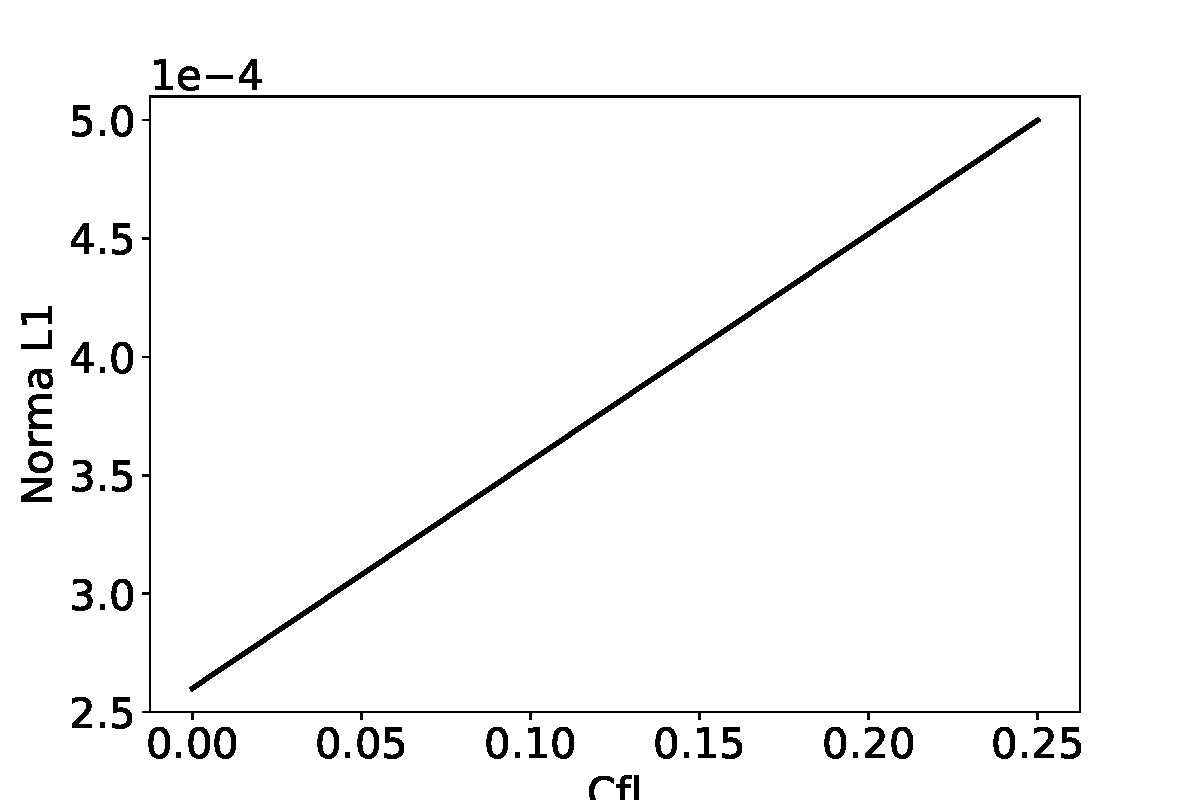
\includegraphics[scale=0.3]{L1}
		\label{fig:erro}
	\end{subfigure}
	\begin{subfigure}[t]{0.3\textwidth}
		\centering
		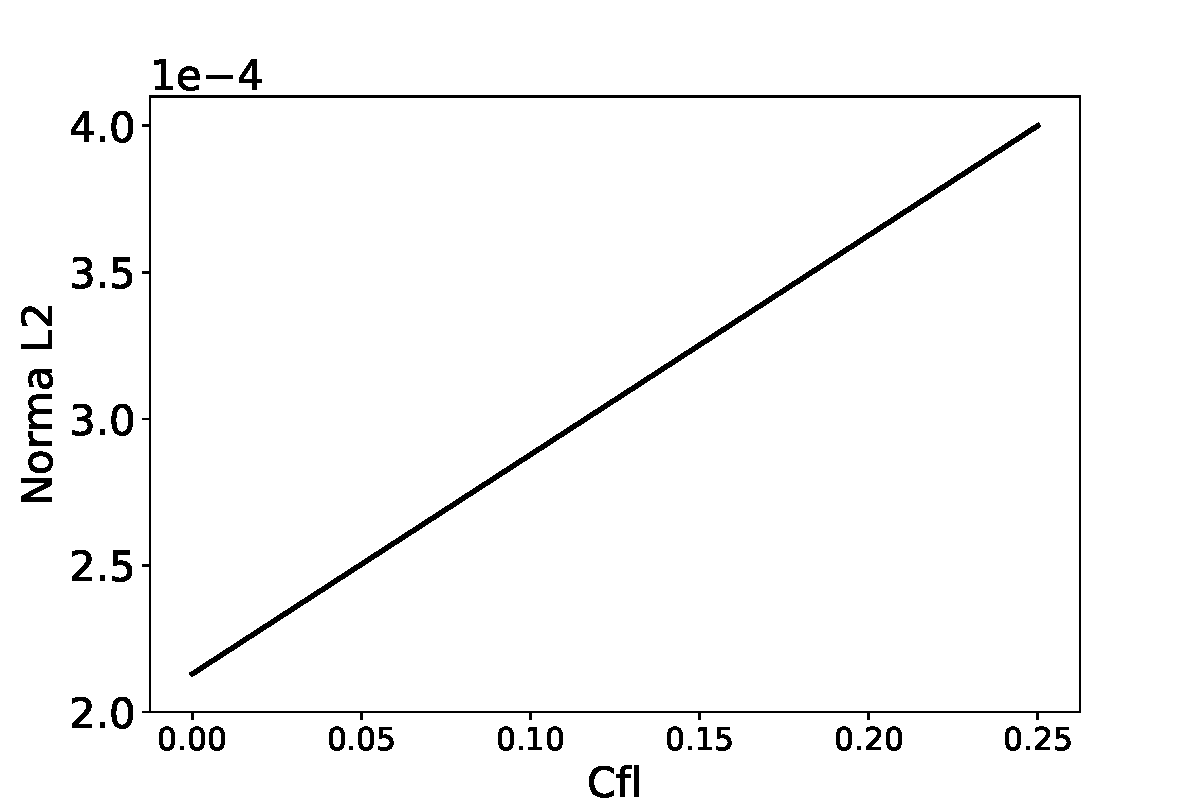
\includegraphics[scale=0.3]{L2}
		\label{fig:erro}
	\end{subfigure}
	\begin{subfigure}[t]{0.3\textwidth}
		\centering
		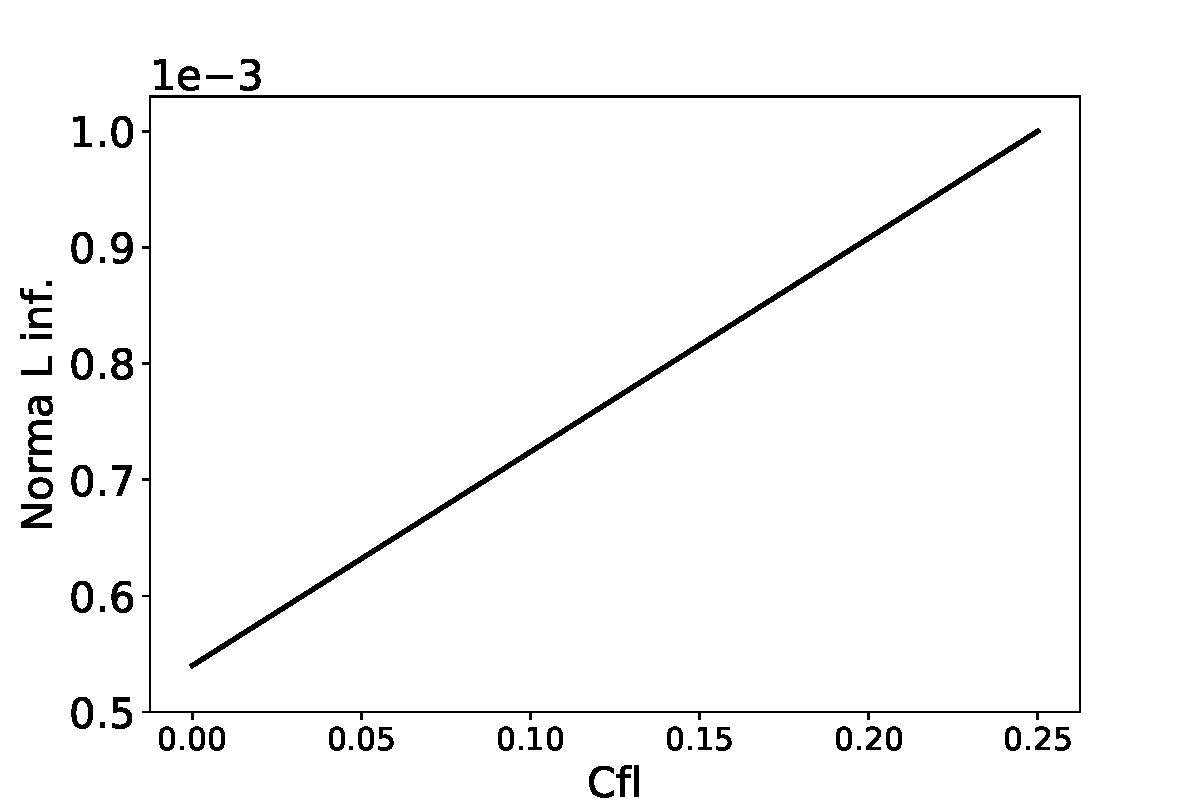
\includegraphics[scale=0.3]{L3}
		\label{fig:erro}
	\end{subfigure}
	\vspace{-5 mm}
	\caption{Erro numérico em função do valor do Cfl.}
	\end{figure*}


	
	\vspace*{-4mm}


	Observa-se na figura 1 que o erro numérico é proporcional ao $CFL$, como esperado pela análise da equação 19.
	
	%==================================
	% CONCLUSÃO
	%==================================
	\section{Conclusão} % apague as linhas abaixo e insira aqui a conclusão
	Propôs-se a avaliação de erro para a solução numérica da equação diferencial parcial parabólica que modela o fenômeno da difusão bidimensional em regime transiente. Utilizou-se o método de Euler explícito para a derivada parcial temporal e diferenças centradas para a espacial. Foram feitas a análise numérica do método de discretização e simulações computacionais para avaliar o erro numérico. A solução numérica foi comparada com a solução analítica. Por fim, conclui-se que a parcela de maior representatividade no erro retornado é a do termo de segunda ordem. Ainda, o erro é ampliado em função do aumento da  entre os passos espacial e temporal (definição de $CFL$).
	
	
	%==================================
	% AGRADECIMENTOS
	%==================================
	\section{Agradecimentos} % apague as linhas abaixo e insira aqui os agradecimentos
	
	Os autores gostariam de agradecer à Petrobras, CAPES, FAPEMIG, CNPq, MFLab e à FEMEC/UFU pelo suporte no desenvolvimento do presente trabalho. 
	
	%==================================
	% REFERÊNCIAS
	%==================================
	
	\begin{thebibliography}{9} % apague as linhas abaixo e insira aqui bibliografia
		
		\bibitem{Leveque_parabolic}
		LEVEQUE, R. J. \textbf{Finite difference methods for ordinary and partial differential equations:} steady-state and time-dependent problem. 1. ed. Philadelphia: SIAM, 2007.
		
		\bibitem{Warming}
		WARMING, R., HYETT, B. The modified equation approach to the stability and accuracy analysis of finite-difference methods.	\textbf{Journal of Computational Physics}, California, v. 14, n. 2, p. 159 – 179, 1974.
	
			
		\bibitem{CFL}
		Courant, R., Friedrichs, K., Lewy, H. On the Partial Difference Equations
		of Mathematical Physics.   \textbf{IBM Journal of Research and Development}, New York, v. 11, i. 2, 1967 
				
	\end{thebibliography}
	
	%--- FIM ---
\end{document}